\chapter{Benchmarks}

\section{Instantaneous dipole in $H_2$}

\citeauthor{li2005time}\cite{li2005time} employ a time-dependent Hartree-Fock 
apporach in order to study the electronic optical response of molecules 
in intense fields. To be specific, they model the hydrogen molecule $H_2$ 
with a \lstinline{6-311++G(d,p)} basis set, subject to an oscillating field 
of $1.72\times10^13\text{ W} \text{cm}^{-2}$ and $456\text{ nm}$. They find the time-dependent
Hartree-Fock method to be nearly indistinguishable from calculations using the 
full time-dependent Schrödinger equation. We have managed to replicate the 
instantaneous dipole of this simulation of hydrogen.

A \lstinline{6-311++G(d,p)} basis set corresponds to a \lstinline{6-311++Gss} 
basis set in \lstinline{PySCF}, and we can extract it from here,
\begin{python}
molecule = "
    h 0.0 0.0 -0.6948522960236121;
    h 0.0 0.0  0.6948522960236121
    "
basis = "6-311++Gss"
system = construct_pyscf_system_ao(molecule, basis=basis)
\end{python}
The bond length of the Hydrogen molecule is approximately $0.7354\text{ Å}$, converted 
to multiples of Bohr radii here. As the naming suggests, the basis set is a split-valence 
triple-zeta basis set, with one added s-type diffuse function and a set of p-type
polarisation 
functions for each Hydrogen atom\footnote{This would be obvious for a quantum chemist,
but basis set configurations looks like incantantions from a spellbook to a physicist}.

In their simulations \citeauthor{li2005time} have used a linearly polarised and 
spatially homogenous external field, 
\begin{equation}
    \vb{e}(\vb{r}, t) = \vb{E}(t)\sin(\omega t).
\end{equation}
The field envelope $|\vb{E}|$ is linearly increased with time to a maximum value 
$|\vb{E}_\text{max}|$ at the end of the first cycle and remains at $|\vb{E}_\text{max}|$
for one cycle and then decreases linearly to zero by the end of the next cycle,
\begin{equation}
    \begin{aligned}
        \vb{E}(t) = (\omega t / 2\pi) \vb{E}_\text{max} \quad &\text{for} \quad
            0 \leq t \leq 2\pi / \omega \\ 
        \vb{E}(t) = \vb{E}_\text{max} \quad &\text{for} \quad 
            2\pi / \omega \leq t \leq 4\pi / \omega \\ 
        \vb{E}(t) = (3 - \omega t / 2\pi) \vb{E}_\text{max} \quad &\text{for} \quad 
            4\pi / \omega \leq t \leq 6\pi / \omega \\
        \vb{E}(t) = 0 \quad &\text{for} \quad
            t < 0 \text{ and } t > 6\pi / \omega,
    \end{aligned}
\end{equation}
where the maximum field intensity if $1.72\times10^14 \text{ W} \text{cm}^{-2}$ 
($E_\text{max} = 0.07 \text{ au}$). \citeauthor{li2005time} also run a simulation 
for a lower intensity, but we are conecerned only with this relatively more intensive 
pulse. The entire simulation lasts for $T=225 \text{ au}$.

The result of our simulation is shown in \autoref{fig:li_compare}, where we have 
computed the instantaneous dipole over time using three different methods. The 
time-dependent Hartre-Fock result is shown in the bottom sub-figure, and is expected 
to be exactly the same as figure 4.a from \citeauthor{li2005time}\cite{li2005time},
which it appear to be. For comparrison we have computed the result with both of 
our time-dependent coupled cluster methods. The result of the time-dependent 
coupled cluster method with single and double excitations are showed in the top subfigure,
and the result of the orbital-adaptive coupled cluster method with double excitations 
are shown in the middel subfigure. We see that there is no perceptible difference between 
the results of the three methods.

\begin{figure}
    \centering
    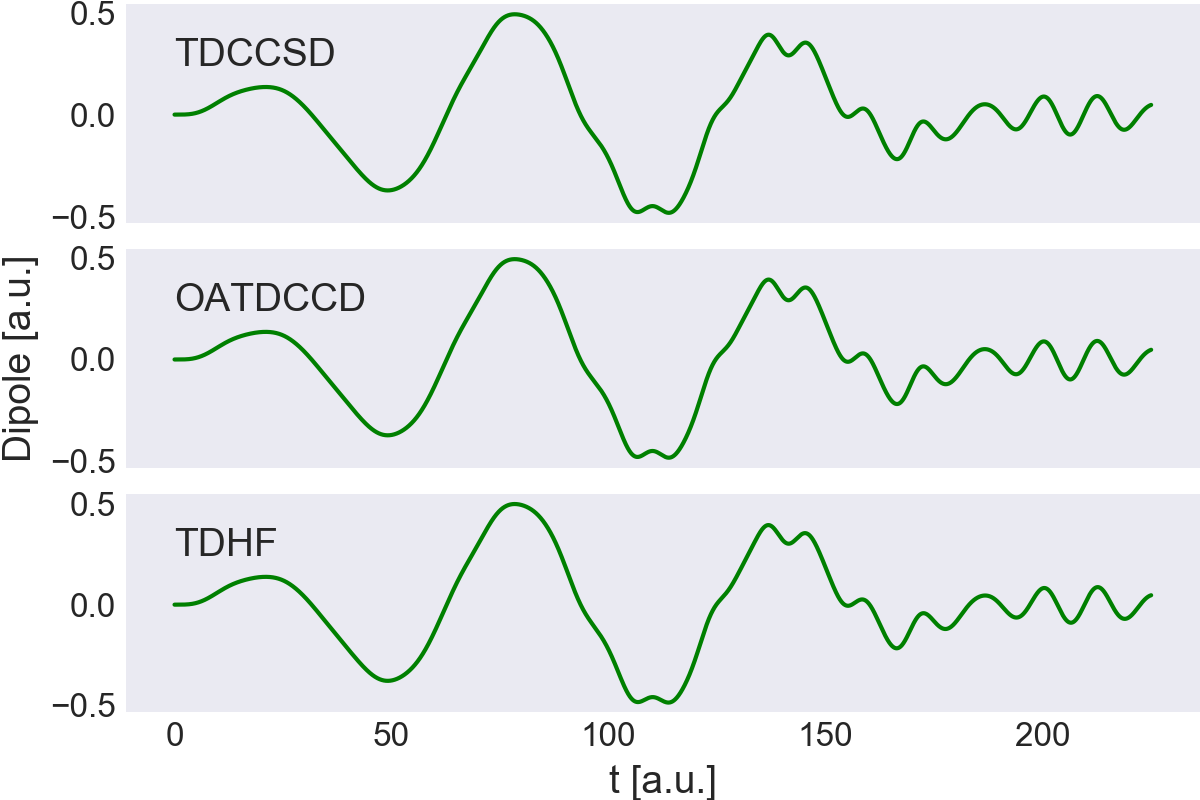
\includegraphics[width=0.75\textwidth]{results/figures/li_compare.png}
    \caption{Instantaneous dipole for $H_2$ in an oscillating electric field
        $E_\text{max} = 0.07 \text{ au}$ ($1.72\times10^14 \text{ W} \text{cm}^{-2}$)
        and $\omega=0.1 \text{ au}$ ($456\text{ nm}$) using a \lstinline{6-311++G(d,p)}
        basis set.
    }
    \label{fig:li_compare}
\end{figure}


\section{Zanghellini}

Zanghellini et al.\cite{Zanghellini04} calculate the time development of a 
one-dimensional quantum dot with two electrons using the multi-configurational 
time-dependent Hartree-Fock method (MCTDHF). This method yields excact results for 
a very large number of configurations, $\eta \to \infty$. This study would provide a 
proper benchmark for our implementation because the coupled cluster method with singles and 
doubles excitations (CCSD) is excact for $n=2$ particles. 
The harmonic oscillator potential applied in
their study had a frequency of $\omega=0.25$, used a strong laser-like field with 
maximum intensity of $E = 1$ and a laser frequency of $\Omega = 8 \omega = 2$.
Their MCTDHF scheme convergences with $\eta=15$
configurations up to the resulotion of their figures.
We are able to reproduce their results precisesly by employing the 
time-dependent coupled cluster method with singles and double excitations (TDCCSD) with 
static orbitals, using $l=20$ spin-orbitals in the basis set.

In \autoref{fig:zanghellini_fig1} we see the ground state electron density for the 
ground state wavefunction computed with CCSD. Zanghellini et al. computed the electron
density for an increasing number of configurations $\eta$ using multi-configurational
Hartree-Fock (MCHF). This figure matches the convergent electron density found by Zanghellini et al. 
as $\eta \to \infty$, in figure 1 from their article. 

\begin{figure}
    \centering
    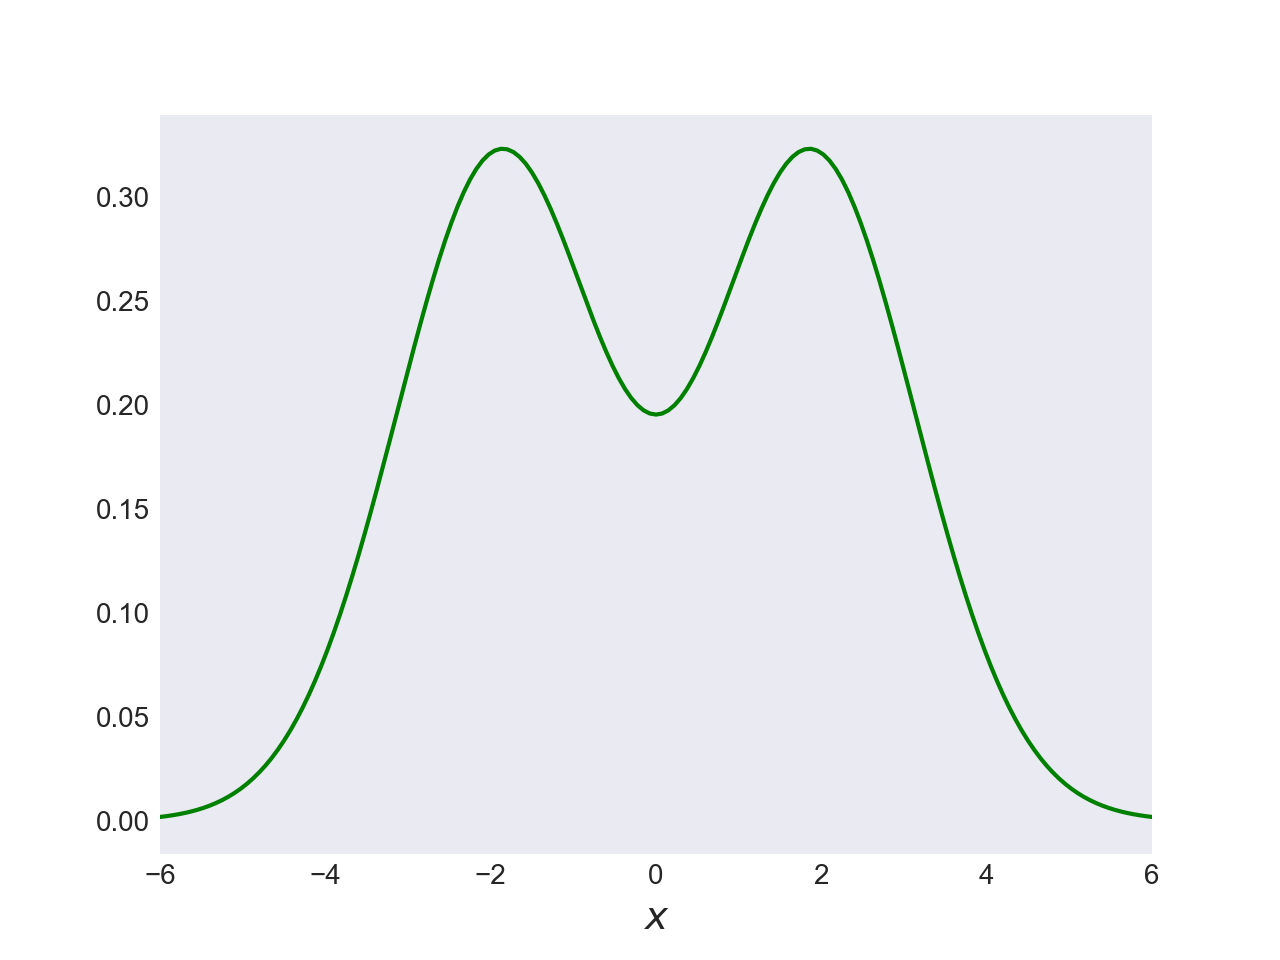
\includegraphics[width=0.75\textwidth]{results/figures/zanghellini_fig1.png}
    \caption{
        \label{fig:zanghellini_fig1}
        Electron density for the ground state wavefunction of a quantum dot with 
        $n=2$ eletrons and $l=20$ spin-orbitals in the basis set computed with
        CCSD. This plot 
        corresponds precisely with figure 1 in Zanghellini et al.\cite{Zanghellini04}.
    }
\end{figure}

\autoref{fig:zanghellini_fig2} depicts the probability fo the system being in the ground 
state as a function of time. Here we have included both a time-dependent Hartree-Fock
computation, corresponding to a MCTDHF computation with $\eta=1$ configurations, and 
a TDCCSD computation, corresponding to MCTDHF when $\eta\to\infty$. We find that our plots
matches Zanghellin et ali's plots in their figure 2 precicely. 

\begin{figure}
    \centering
    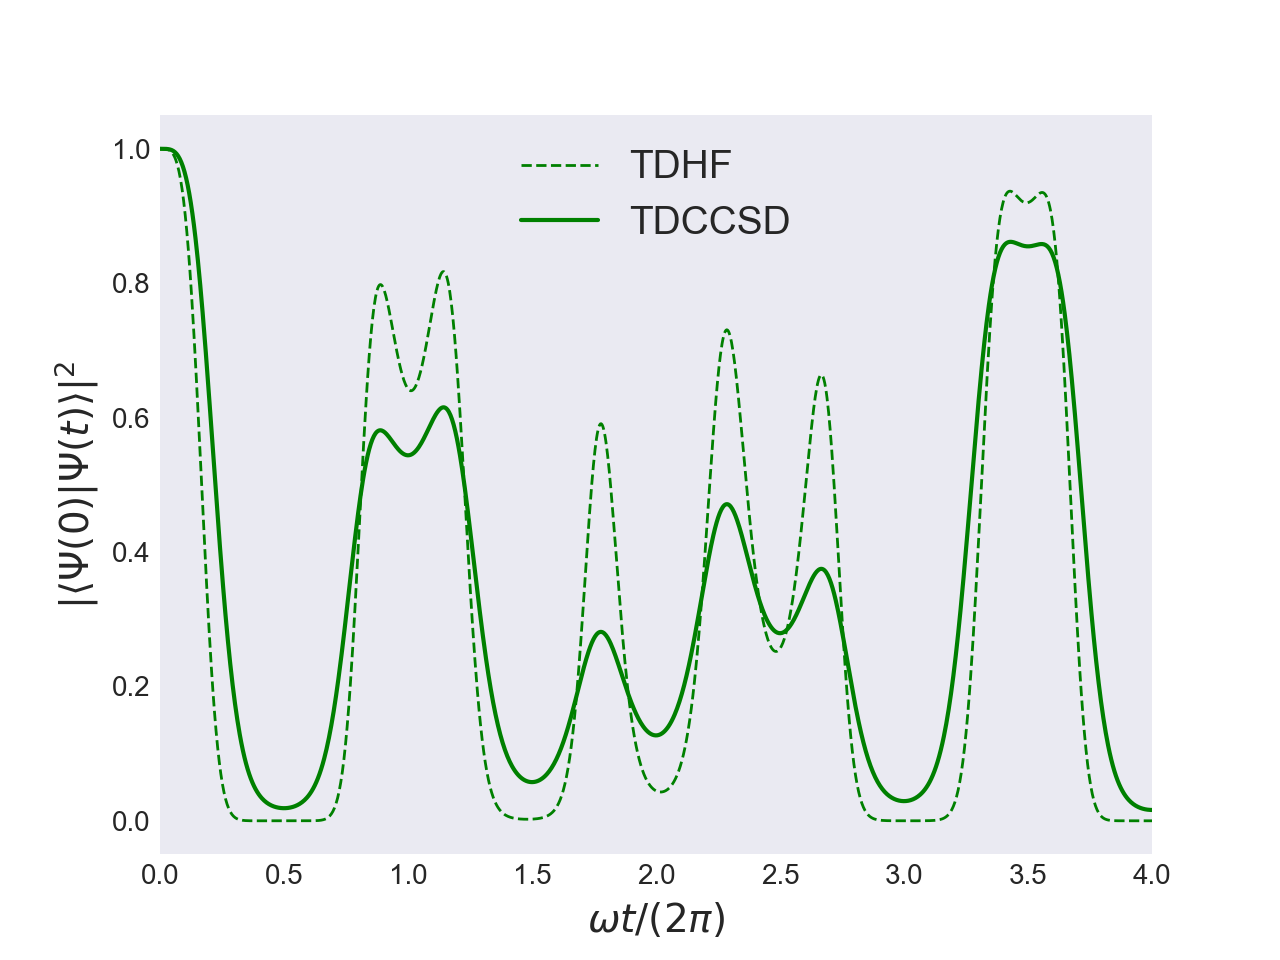
\includegraphics[width=0.75\textwidth]{results/figures/zanghellini_fig2.png}
    \caption{
        \label{fig:zanghellini_fig2}
        Probability of being in the ground state $|\braket{\Phi(0)}{\Phi(t)}|$
        using both TDHF and TDCCSD, for a one-dimensional quantum dot with $n=2$
        particles and $l=20$ spin-orbitals. This plot corresponds precisely with 
        figure 2 in Zanghellini el al.\cite{Zanghellini04}.
    }           
\end{figure}